%!TEX root = ../uwo.tex

\begin{frame}[plain,noframenumbering]
	\centering
	\vspace*{2.6cm}
	\Huge \colorit{Part III}
	\vskip 20pt
	\Large Persistence cohomology
\end{frame}

\begin{frame}{Goal: introduce Steenrod barcodes}
	\pause
	These generalize usual barcodes, and are also
	\pause
	\colorit{stable},
	\pause
	\colorit{computable},
	\pause
	and present in \colorit{real-data}.

	\pause\medskip
	\vskip-15pt
	\begin{figure}
		\centering
		\begin{subfigure}[b]{0.49\textwidth}
			\centering
			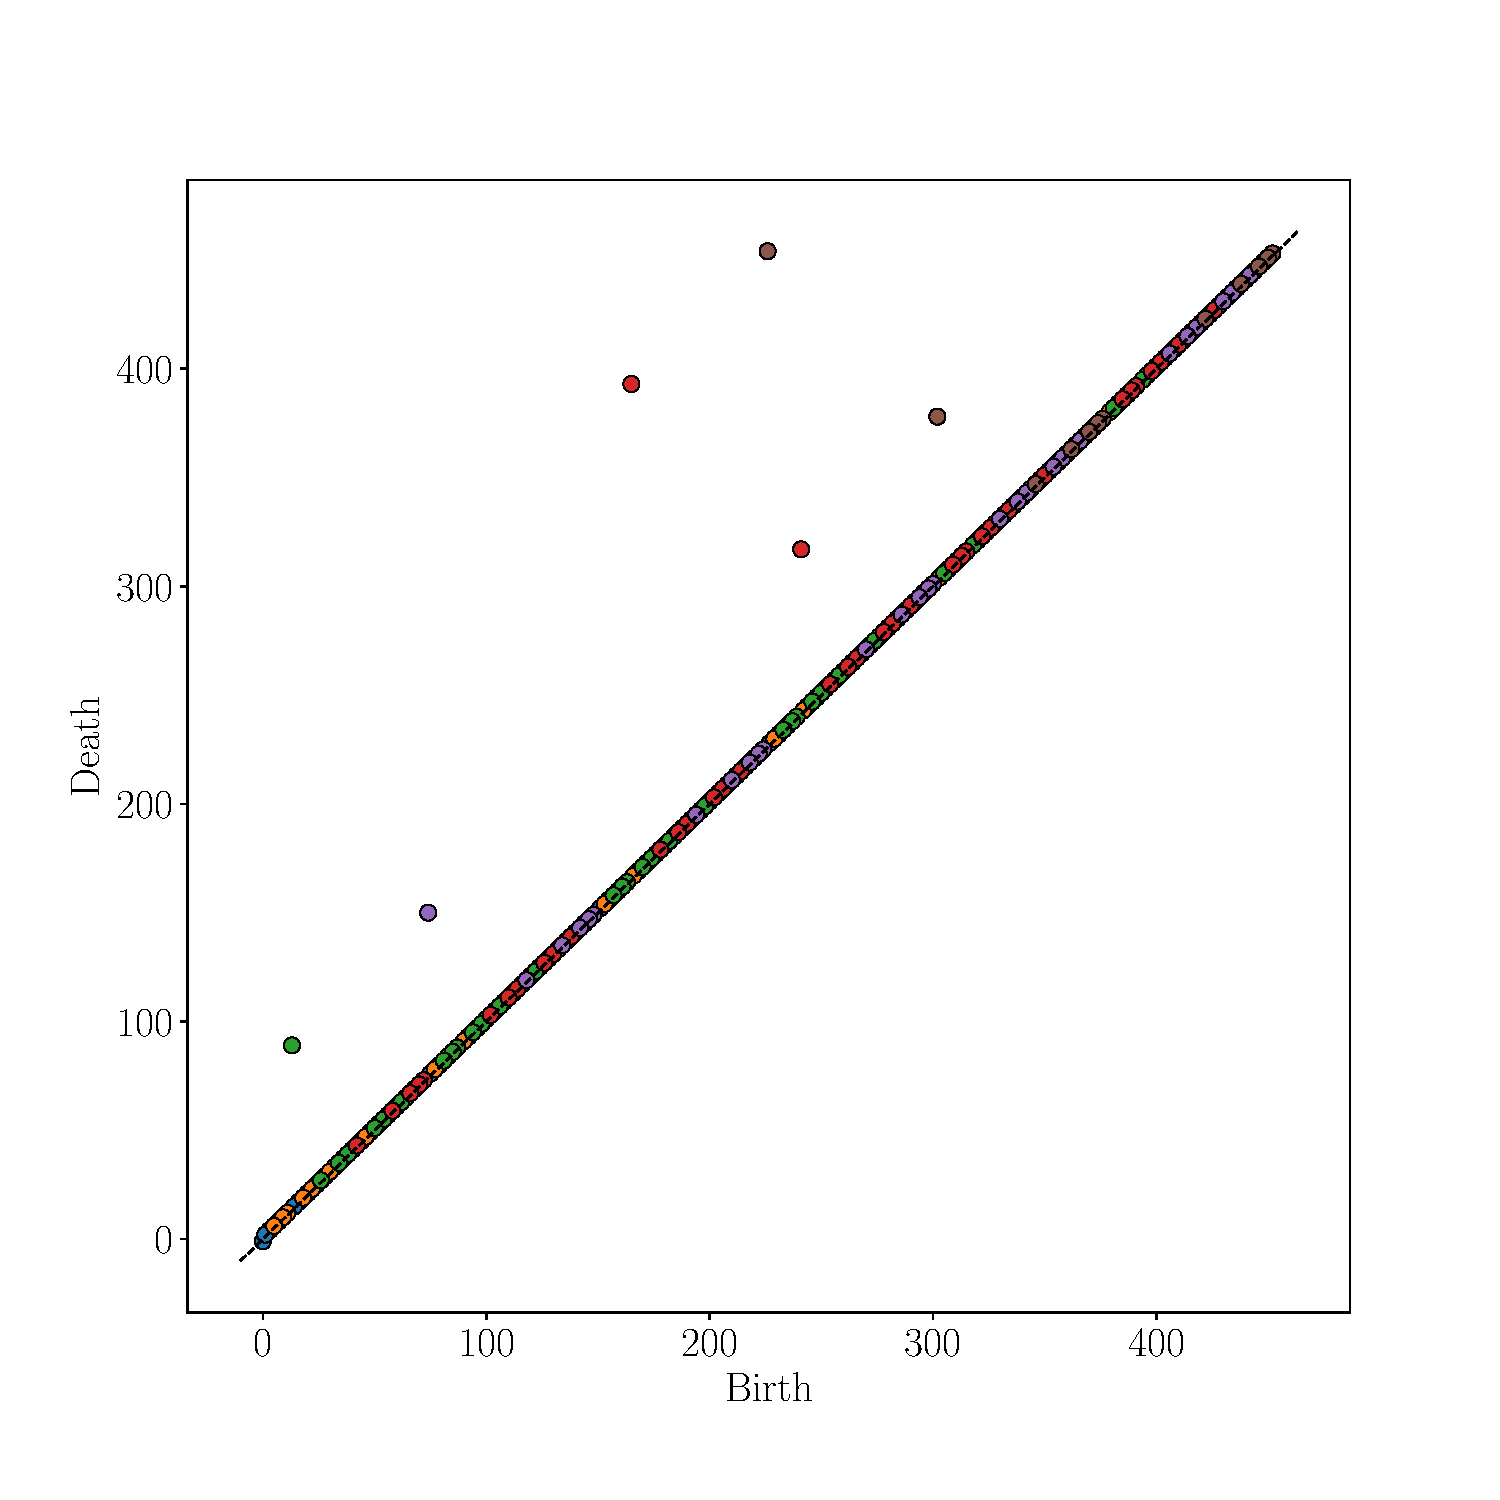
\includegraphics[width=\textwidth]{aux/s2_s4.pdf}
			\caption{$\mathrm C\,\Sigma(S^2 \vee S^4)$}
			\label{f:s2_s4}
		\end{subfigure}
		\pause
		\begin{subfigure}[b]{0.49\textwidth}
			\centering
			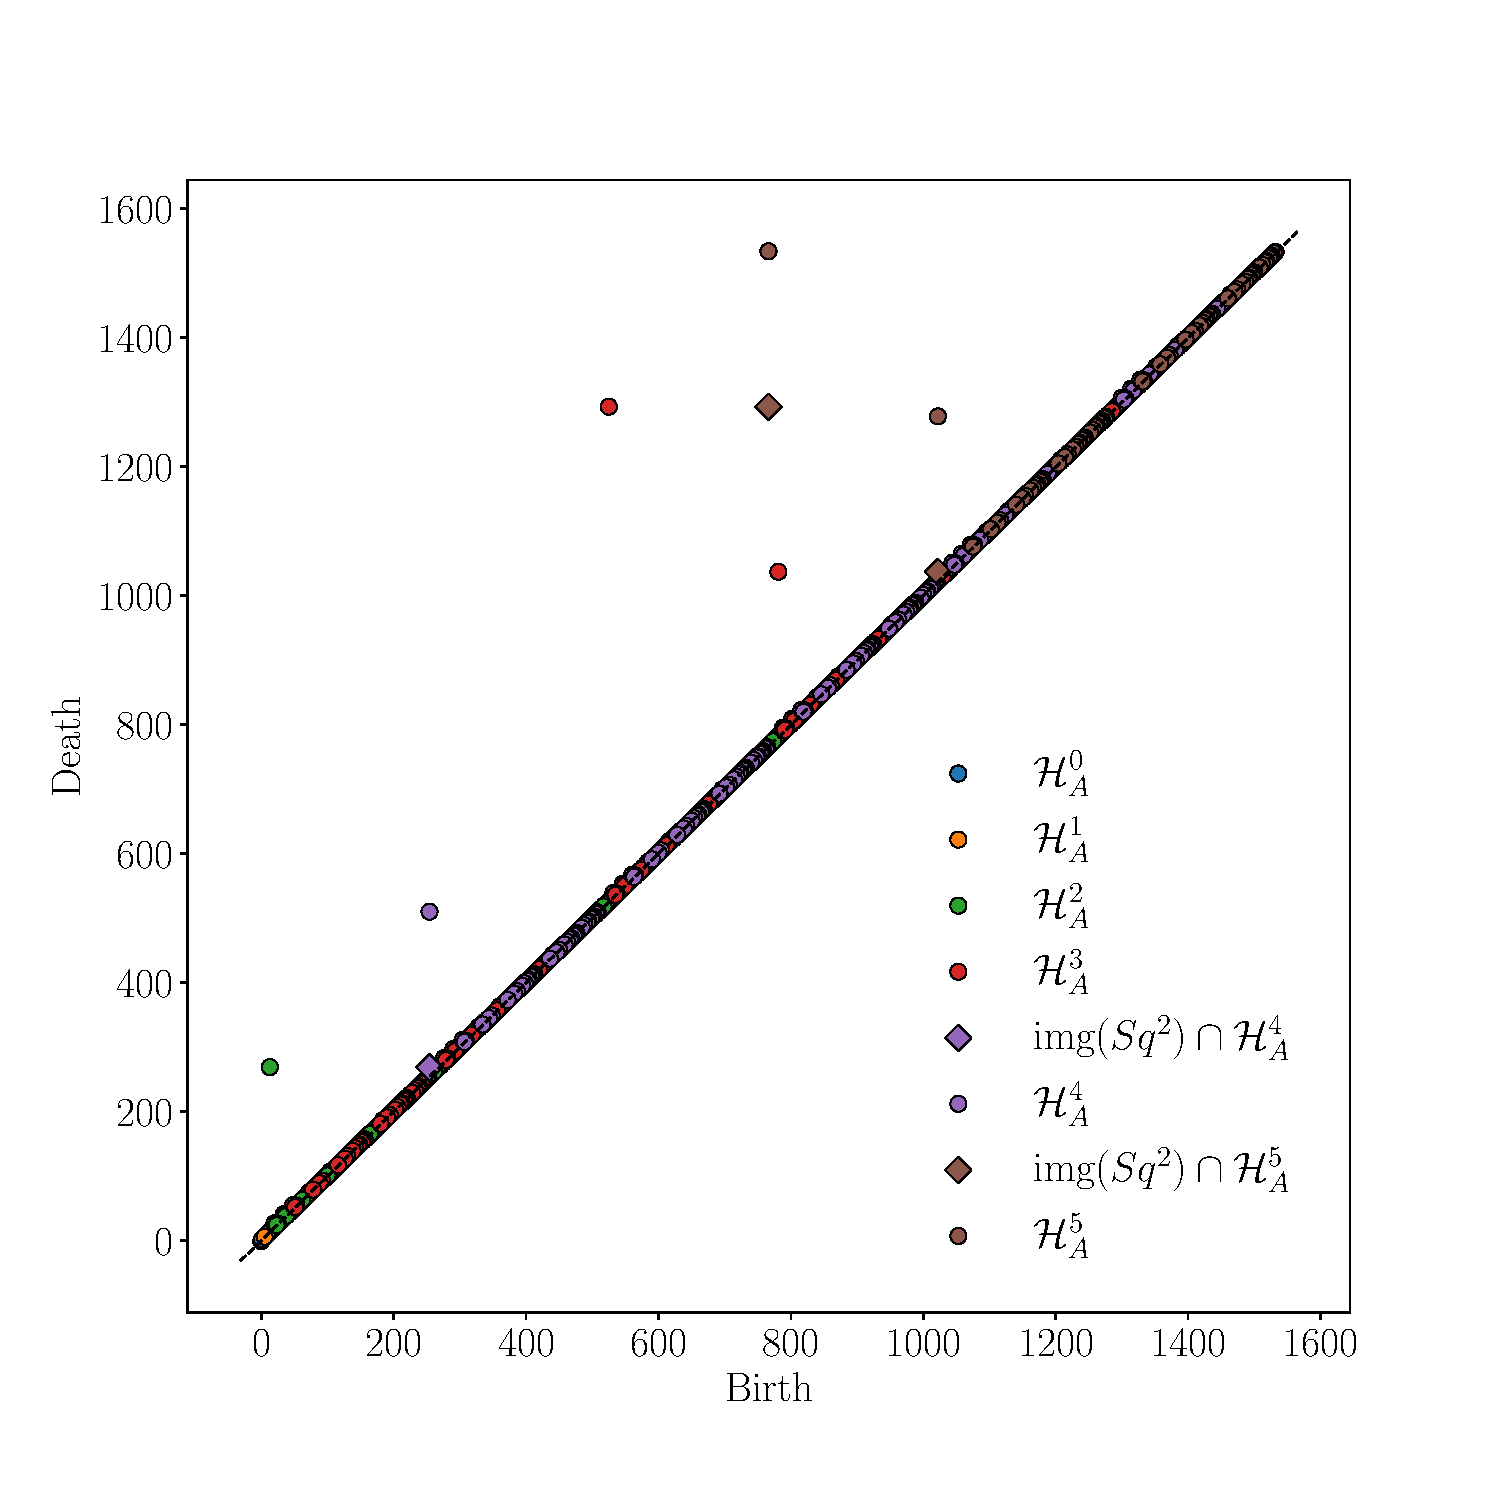
\includegraphics[width=\textwidth]{aux/cp2.pdf}
			\caption{$\mathrm C\,\Sigma\,\mathbb C \mathrm P^2$}
			\label{f:cp2}
		\end{subfigure}
	\end{figure}
\end{frame}

\begin{frame}{Shortcomings of Betti numbers}
	\pause
	Barcodes are based on the \colorit{Betti numbers} of spaces.

	\pause\bigskip
	But these \colorit{forget} much information.

	\pause\bigskip
	As graded \colorit{vector spaces}
	\[
	H^\bullet(\R \rP^2; \Ftwo) \cong H^\bullet(S^1 \vee S^2; \Ftwo).
	\]

	\pause
	Similarly, as graded \colorit{abelian groups}
	\[
	H^\bullet(\bC \rP^2; \Z) \cong H^\bullet(S^2 \vee S^4; \Z).
	\]

	\pause
	As graded \colorit{rings}
	\[
	H^\bullet(\Sigma(\bC \rP^2)) \cong H^\bullet(\Sigma(S^2 \vee S^4)),
	\]

	\pause\medskip
	As \colorit{modules} over the \colorit{Steenrod algebra}.
	\[
	H^\bullet(\Sigma(\bC \rP^2)) \not\cong H^\bullet(\Sigma(S^2 \vee S^4)),
	\]
\end{frame}

\begin{frame}{Intuition}
	\pause
	\begin{figure}
		\newcommand*{\xMin}{0}%
\newcommand*{\xMax}{4}%
\newcommand*{\yMin}{0}%
\newcommand*{\yMax}{4}%
%\only<2>{
%\vskip4pt
%\begin{center}
%	\centering
%	\begin{tikzpicture}[scale=.6]
%		\draw[-{Latex[length=2mm]}] (-.5,\yMin)--(-.5,\yMax);
%		\draw[-{Latex[length=2mm]}] (-.5,\yMin)--(-.5,\yMax-.5);
%		\draw[-{Latex[length=2mm]}] (4.5,\yMin)--(4.5,\yMax);
%		\draw[-{Latex[length=2mm]}] (4.5,\yMin)--(4.5,\yMax-.5);
%
%		\draw[-{Latex[length=2mm]}] (\xMin, -.5)--(\xMax, -.5);
%		\draw[-{Latex[length=2mm]}] (\xMin, 4.5)--(\xMax, 4.5);
%
%		\draw (0,0)--(0,4)--(4,4)--(4,0)--(0,0);
%
%		\node at (2,5.3){Torus};
%		\node at (2,-1.3){\phantom{$\rank \Sq^1 = 0$}};
%	\end{tikzpicture}
%	\hspace*{2cm}
%	\begin{tikzpicture}[scale=.6]
%		\draw[-{Latex[length=2mm]}] (-.5,\yMin)--(-.5,\yMax);
%		\draw[-{Latex[length=2mm]}] (-.5,\yMin)--(-.5,\yMax-.5);
%		\draw[-{Latex[length=2mm]}] (4.5,\yMax)--(4.5,\yMin);
%		\draw[-{Latex[length=2mm]}] (4.5,\yMax)--(4.5,\yMin+.5);
%
%		\draw[-{Latex[length=2mm]}] (\xMin, -.5)--(\xMax, -.5);
%		\draw[-{Latex[length=2mm]}] (\xMin, 4.5)--(\xMax, 4.5);
%
%		\draw (0,0)--(0,4)--(4,4)--(4,0)--(0,0);
%
%		\node at (2,5.3){Klein Bottle };
%		\node at (2,-1.3){\phantom{$\rank \Sq^1 = 1$}};
%	\end{tikzpicture}
%	%	\caption{Klein Bottle. $\rank \Sq^1 = 0$}
%\end{center}}
\pause
\begin{center}
	\centering
	\begin{tikzpicture}[scale=.6]
		\draw[-{Latex[length=2mm]}] (-.5,\yMin)--(-.5,\yMax);
		\draw[-{Latex[length=2mm]}] (-.5,\yMin)--(-.5,\yMax-.5);
		\draw[-{Latex[length=2mm]}] (4.5,\yMin)--(4.5,\yMax);
		\draw[-{Latex[length=2mm]}] (4.5,\yMin)--(4.5,\yMax-.5);

		\draw[-{Latex[length=2mm]}] (\xMin, -.5)--(\xMax, -.5);
		\draw[-{Latex[length=2mm]}] (\xMin, 4.5)--(\xMax, 4.5);

		\draw (0,0)--(0,4)--(4,4)--(4,0)--(0,0);

		\draw[color=blue!50, very thick] (0,2) .. controls (1,2.5) and (3,1.5) .. (4,2);
		\draw[color=red!50, very thick] (0,1) .. controls (1,1.3) and (3,1) .. (4,1);

		\node at (2,5.3){$T$};
		\node at (2,-1.3){$\rank \Sq^1 = 0$};
	\end{tikzpicture}
	\hspace*{2cm}
	\begin{tikzpicture}[scale=.6]
		\draw[-{Latex[length=2mm]}] (-.5,\yMin)--(-.5,\yMax);
		\draw[-{Latex[length=2mm]}] (-.5,\yMin)--(-.5,\yMax-.5);
		\draw[-{Latex[length=2mm]}] (4.5,\yMax)--(4.5,\yMin);
		\draw[-{Latex[length=2mm]}] (4.5,\yMax)--(4.5,\yMin+.5);

		\draw[-{Latex[length=2mm]}] (\xMin, -.5)--(\xMax, -.5);
		\draw[-{Latex[length=2mm]}] (\xMin, 4.5)--(\xMax, 4.5);

		\draw (0,0)--(0,4)--(4,4)--(4,0)--(0,0);

		\draw[color=blue!50, very thick] (0,2) .. controls (1,2.5) and (3,1.5) .. (4,2);
		\draw[color=red!50, very thick] (0,1) .. controls (1,1) and (2,2.5) .. (4,3);

		\node at (2,5.3){$K$};
		\node at (2,-1.3){$\rank \Sq^1 = 1$};
	\end{tikzpicture}
%	\caption{Klein Bottle. $\rank \Sq^1 = 0$}
\end{center} % REMEMBER TO UNCOMMENT INSIDE
	\end{figure}

	\pause\bigskip
	\colorit{Question}: How to compute the product and Steenrod action in practice.
\end{frame}

\begin{frame}{Cup-$i$ coproducts}
	\pause
	We need \colorit{explicit} maps
	\[
	\Delta_i \colon \gchains(X) \to \gchains(X)^{\otimes 2}
	\quad \text{satisfying} \quad
	\partial \Delta_{i} = \big(1 \pm T \big) \Delta_{i-1}
	\]

	\pause\bigskip\smallskip
	Then, the \colorit{product} is
	\[
	\begin{split}
		H^\bullet(X) \ot H^\bullet(X) &\to H^\bullet(X) \\
		[\alpha] \ot [\beta] &\mapsto \big[ (\alpha \otimes \beta) \Delta_0(-) \big]
	\end{split}
	\]

	\smallskip\pause
	and the $k^\th$ \colorit{Steenrod square}
	\[
	\begin{split}
		\Sq^k \colon H^\bullet(X; \Ftwo) &\to H^\bullet(X; \Ftwo) \\
		[\alpha] &\mapsto \big[ (\alpha \otimes \alpha) \Delta_{\bars{\alpha}-k}(-) \big]
	\end{split}
	\]
\end{frame}

\begin{frame}{A new description of Steenrod's construction}
	\pause
	\colorit{Definition (Med.)} \\
	For a basis element $x \in \gchains_m(X, \Ftwo)$
	\[
	\textstyle \Delta_i(x) = \sum d_{U^0}(x) \otimes d_{U^1}(x)
	\]
	where the sum is over subsets $U = \{u_1 < \cdots < u_{n-i}\} \subseteq \{0, \dots, n\}$ and
	\begin{equation*} \label{e:partition subsets}
		U^0 = \{u_j \in U\mid u_j \equiv j \text{ mod } 2\}, \qquad
		U^1 = \{u_j \in U\mid u_j \not\equiv j \text{ mod } 2\}.
	\end{equation*}

	\pause\medskip
	\colorit{Theorem (Med.)} \\
	All cup-$i$ constructions in the literature are equal up isomorphism:
	\vskip -7.5pt
	\[
	\triangle \sim \triangle^\prime \iff \forall i \in \N, \ \triangle_i = \triangle_i^\prime \ \vee \, \triangle_i = T \triangle_i^\prime.
	\]
	\vskip -3pt
	(Proven via an axiomatic characterization.)

	\pause\bigskip
	If interesting, we can discuss \colorit{connections} to
	higher category theory, convex and toric geometry, knot theory, and condensed matter physics.
\end{frame}

\begin{frame}{Fast computation of Steenrod squares}
	\pause
	Comparing with SAGE: (algorithm based on EZ-AW contraction)

	\smallskip\pause
	\colorit{$\Sq^1$} on \colorit{$\Sigma^i\R P^2$} ($i^\th$ suspension of the real projective plane)

	\medskip
	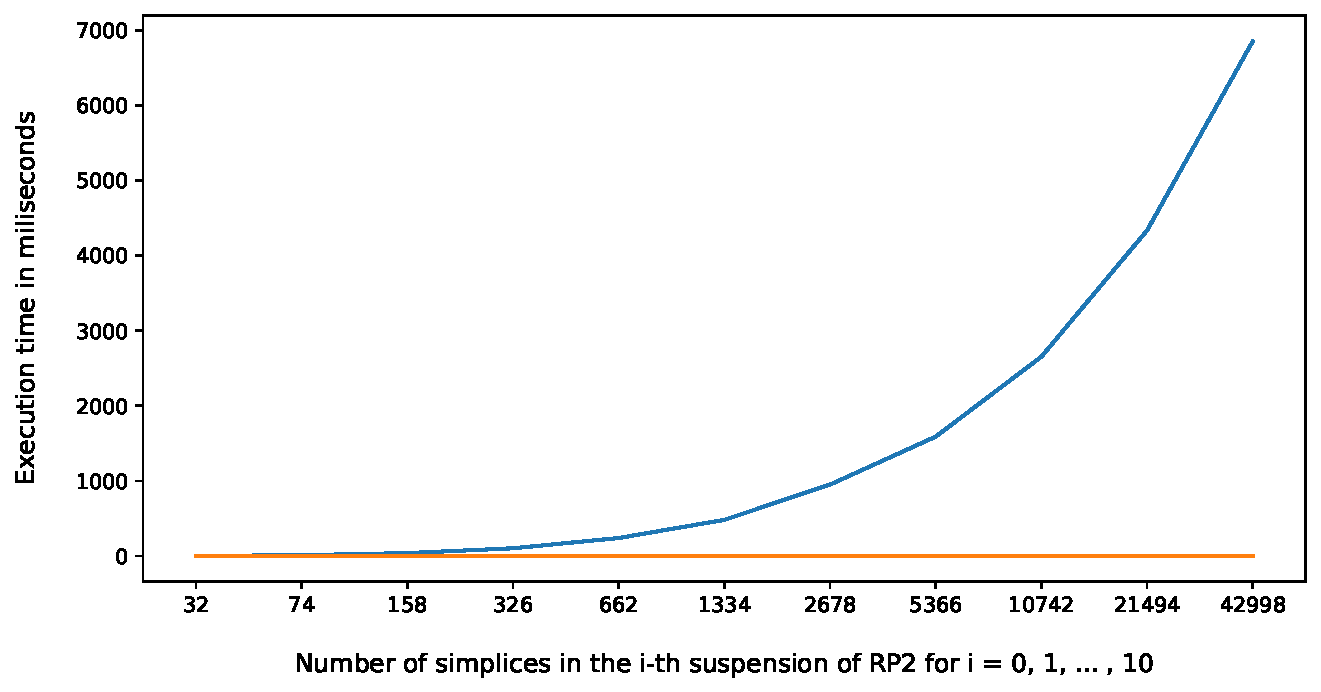
\includegraphics[width=\textwidth]{aux/comp_sus_rp2.pdf}
\end{frame}

\begin{frame}[fragile]{Steenrod barcodes}
	\pause
	Given
	\begin{equation}\label{eq:filtration}
		X_0 \to X_1 \to \cdots \to X_n,
	\end{equation}

	\pause\smallskip
	$\Sq^k$ induces an \colorit{endomorphism}
	\[
	\begin{tikzcd}[column sep = 15]
		H^\bullet(X_n; \Ftwo) \arrow[r] & \cdots \arrow[r] & H^\bullet(X_{n-1}; \Ftwo) \arrow[r] & H^\bullet(X_0; \Ftwo) \\
		H^\bullet(X_n; \Ftwo) \arrow[u, "\Sq^k"] \arrow[r] & \cdots \arrow[r] & H^\bullet(X_{n-1}; \Ftwo) \arrow[u, "\Sq^k"] \arrow[r] & H^\bullet(X_0; \Ftwo) \arrow[u, "\Sq^k"].
	\end{tikzcd}
	\]

	\pause
	\colorit{Definition (Lupo--Med.--Tauzin)} \\
	The \colorit{$\Sq^k$ barcode} of (1) is defined as the barcode of $\mathrm{img}\ \Sq^k$.

	\pause\bigskip
	\colorit{Theorem (Ling Zhou--Med.--M\'emoli)} \\
	These barcodes are stable.

	\pause\bigskip
	\colorit{Computable}?
\end{frame}

\begin{frame}{\texttt{Steenroder}}
	\pause

	A ready-to-use \colorit{package} for computing Steenrod barcodes.

	\begin{center}
		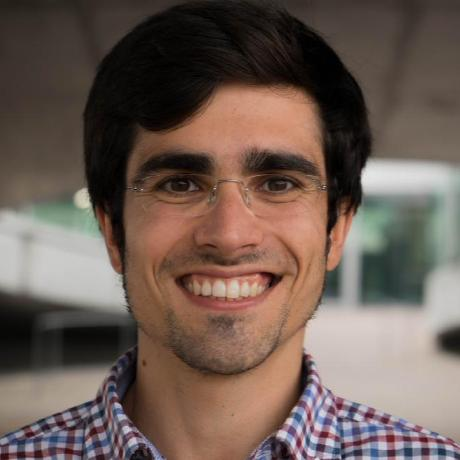
\includegraphics[scale=.1]{aux/umberto}
		\qquad
		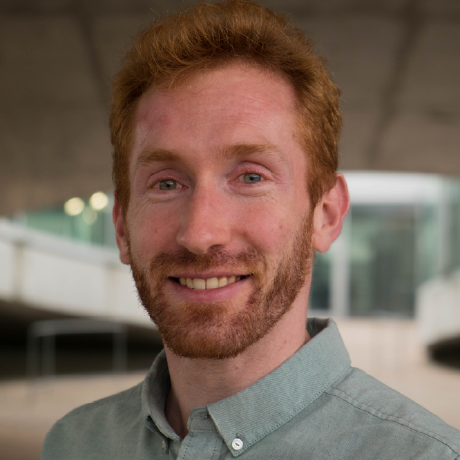
\includegraphics[scale=.1]{aux/guillaume}
	\end{center}

	Developed with \textit{U. Lupo} and \textit{G.~Tauzin} from \raisebox{-1pt}{
\includegraphics[scale=0.1]{aux/giotto}}.

	\begin{center}
		\hyperlink{https.github.com/Steenroder/steenroder.com}{github.com/Steenroder/steenroder}
	\end{center}

	\pause\bigskip
	\colorit{Question:} Are these finer invariants out there in the world?
\end{frame}

\begin{frame}{Example: $\Sq^2$}
	\pause
	Filtrations of the cone on $\Sigma(S^2 \vee S^4)$ and $\Sigma \bC \rP^2$.

	\pause
	\begin{figure}
		\centering
		\begin{subfigure}[b]{0.49\textwidth}
			\centering
			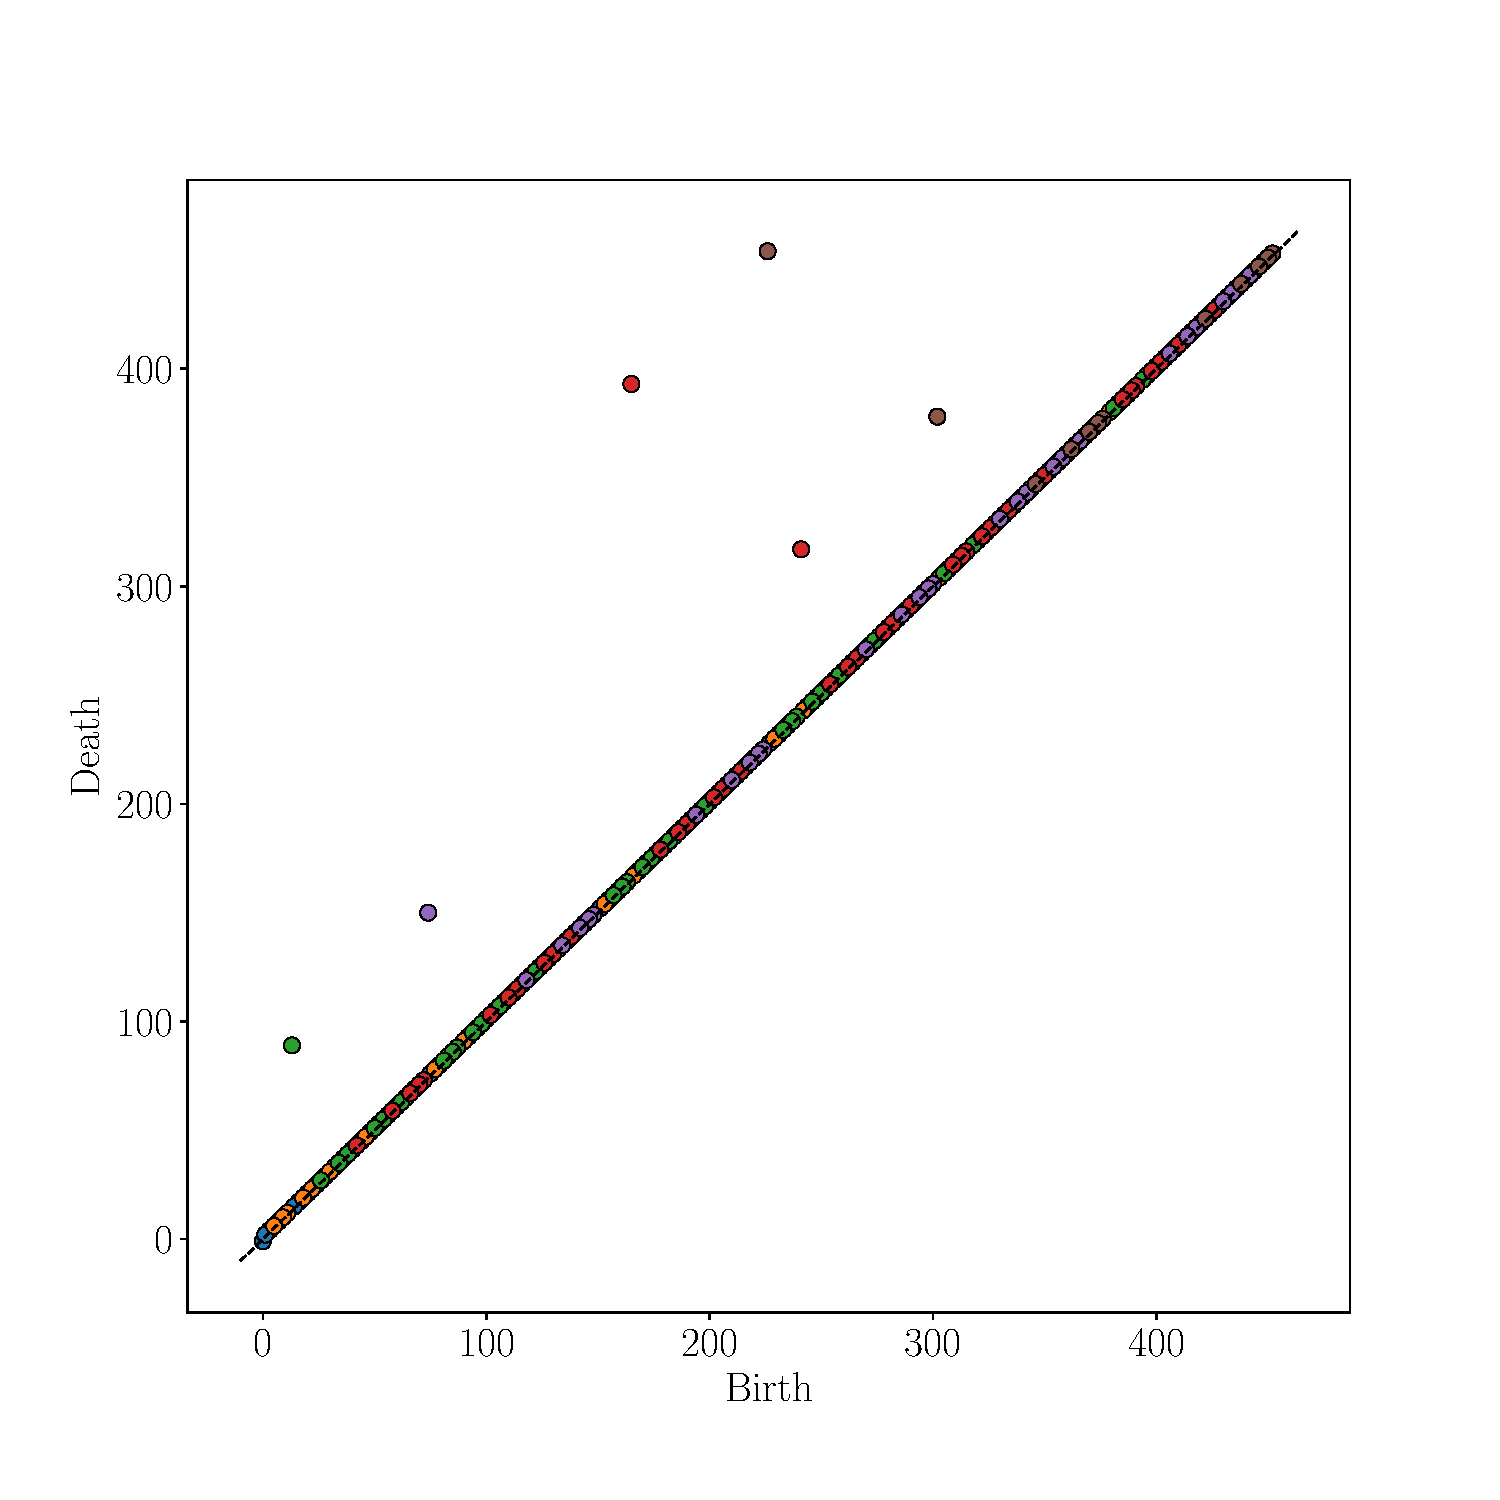
\includegraphics[width=\textwidth]{aux/s2_s4.pdf}
			\caption{$\mathrm C\,\Sigma(S^2 \vee S^4)$}
			\label{f:s2_s4}
		\end{subfigure}
		\begin{subfigure}[b]{0.49\textwidth}
			\centering
			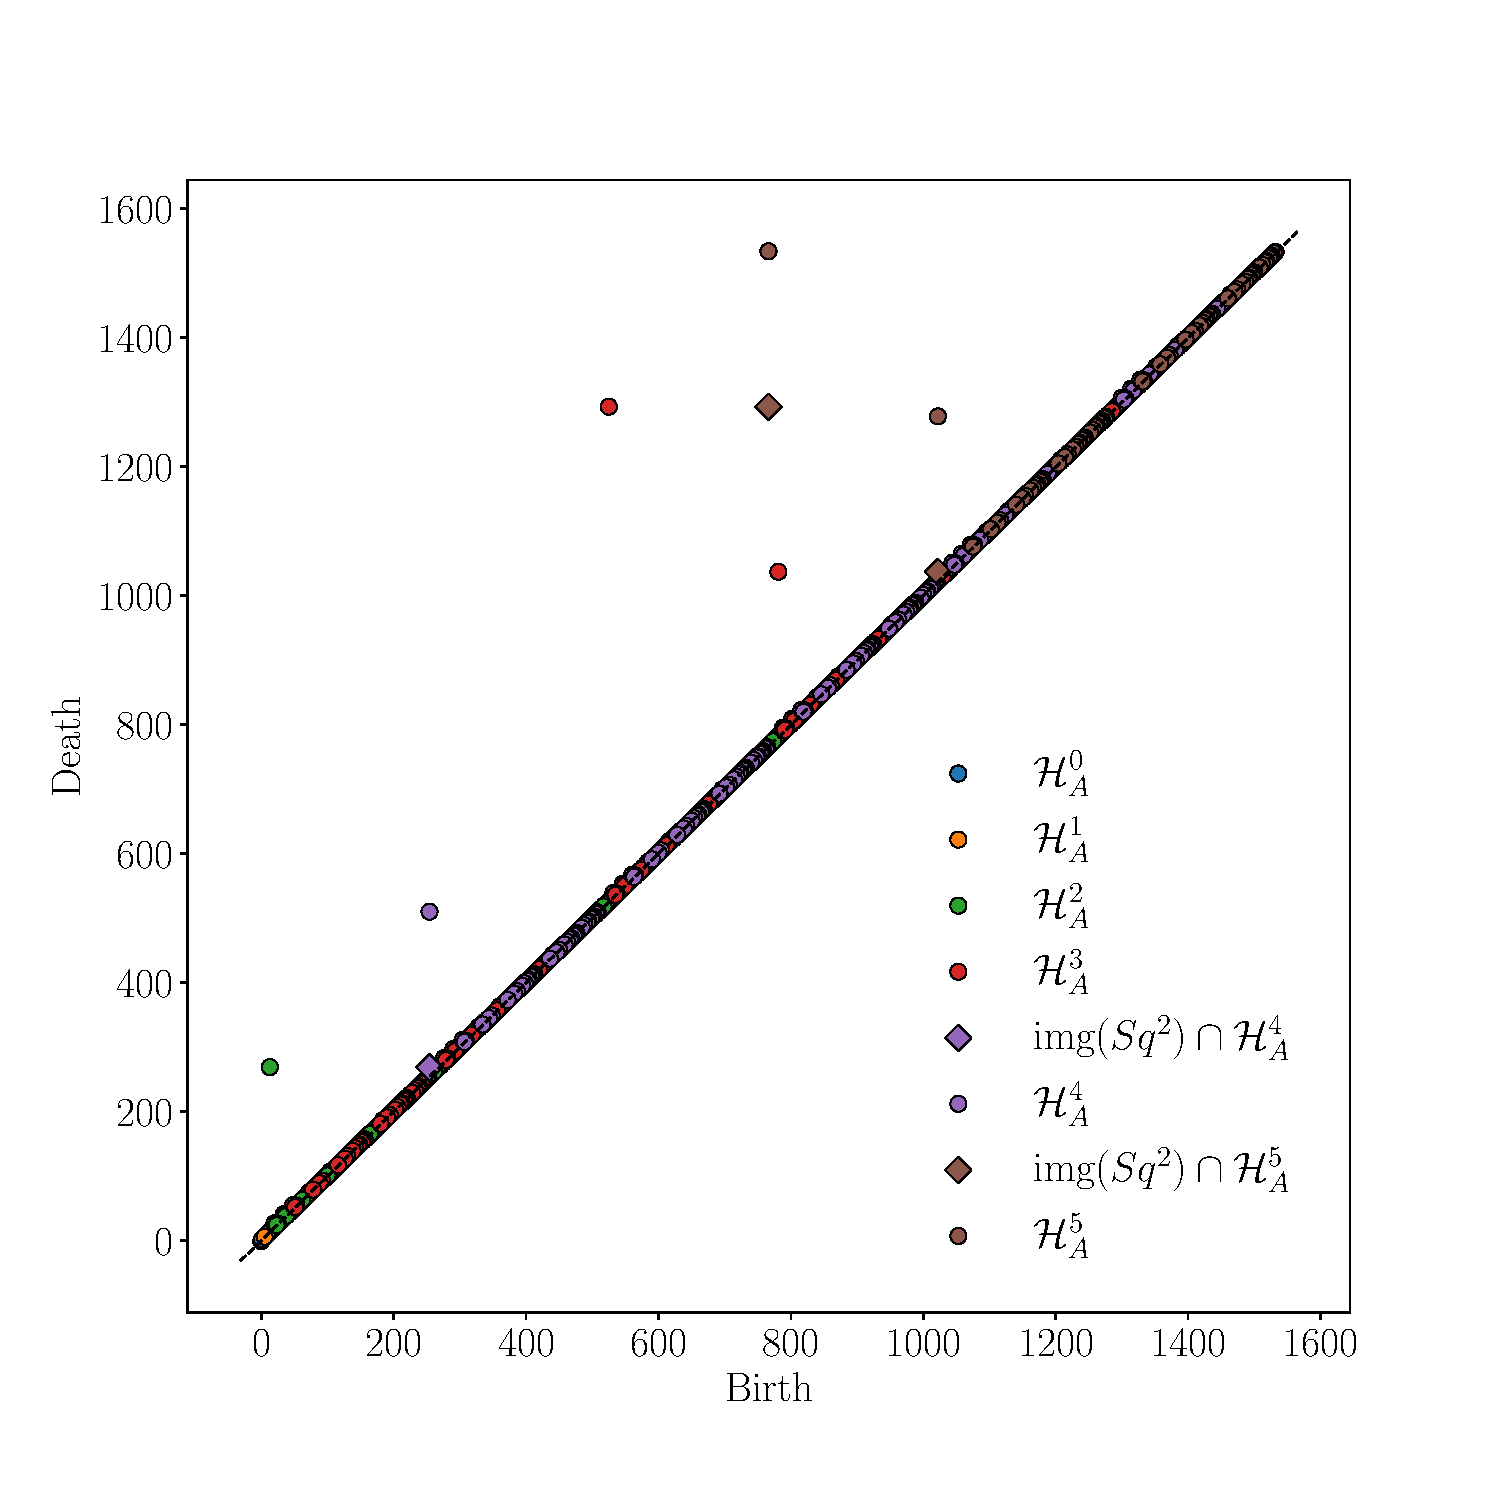
\includegraphics[width=\textwidth]{aux/cp2.pdf}
			\caption{$\mathrm C\,\Sigma\,\bC\rP^2$}
			\label{f:cp2}
		\end{subfigure}
	\end{figure}
\end{frame}

\begin{frame}{Space of conformations of $\mathrm{C_8H_{16}}$}
	\pause
	Points in $\R^{24}$ (positions of $8$ carbons in $\R^3$)

	\pause\medskip
	$H^1$ (green) and $H^2$ (blue) barcodes of (part of) this point cloud
	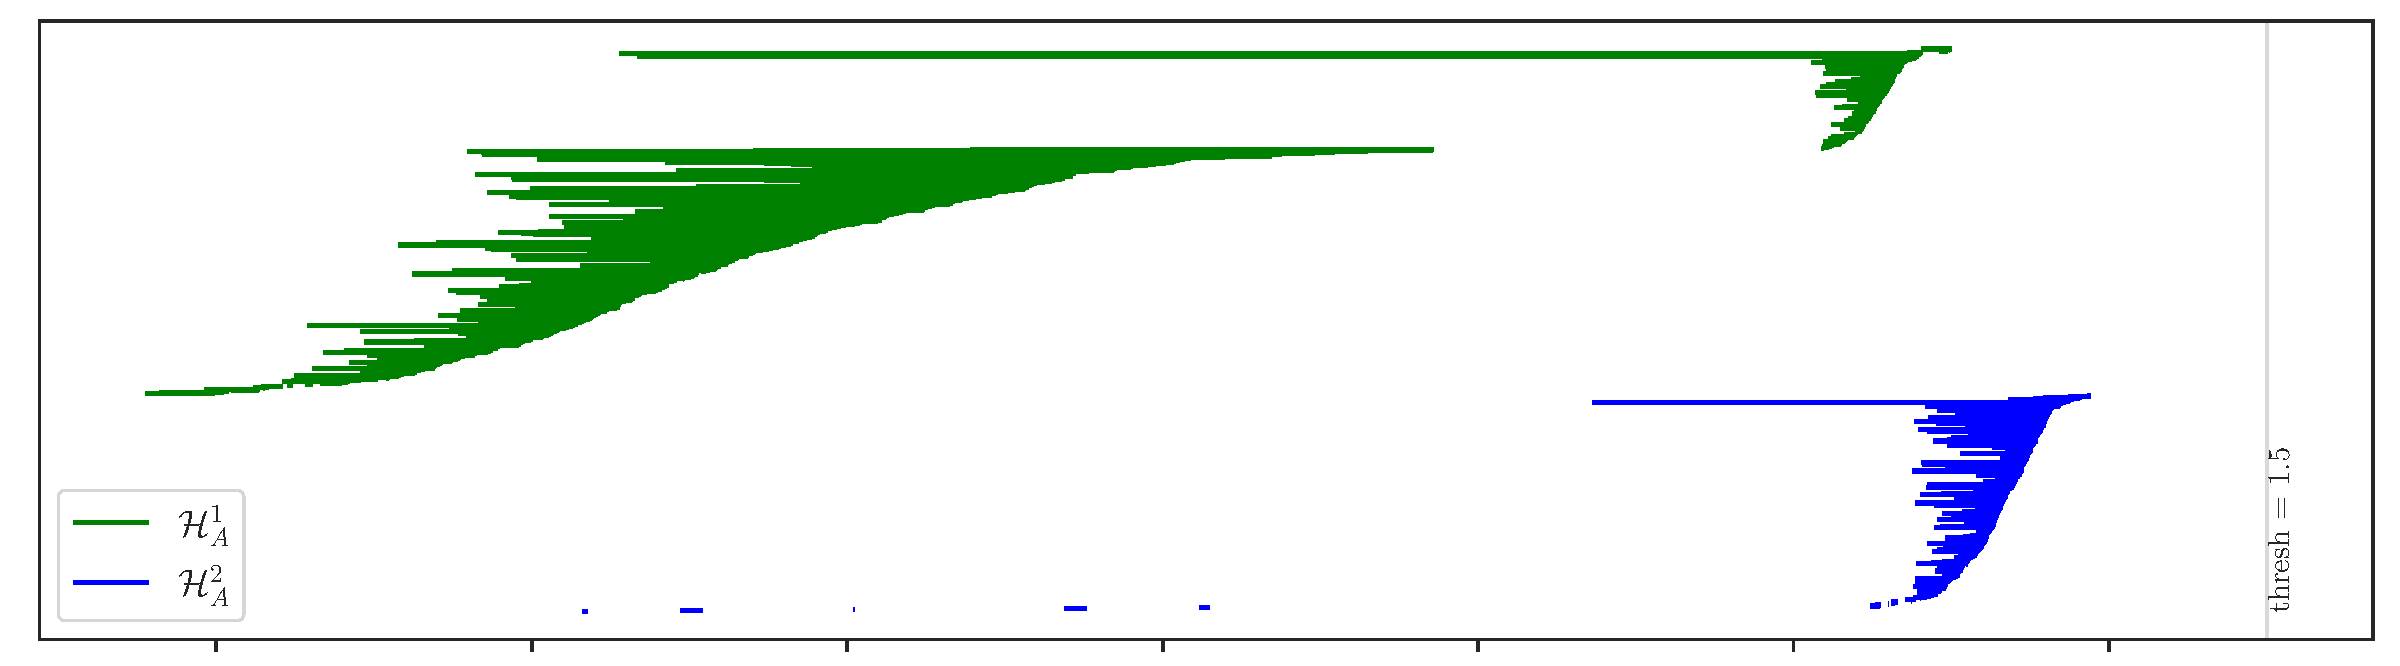
\includegraphics[width=\textwidth]{aux/molecule_top.pdf}

	\pause
	$\Sq^1$ barcode
	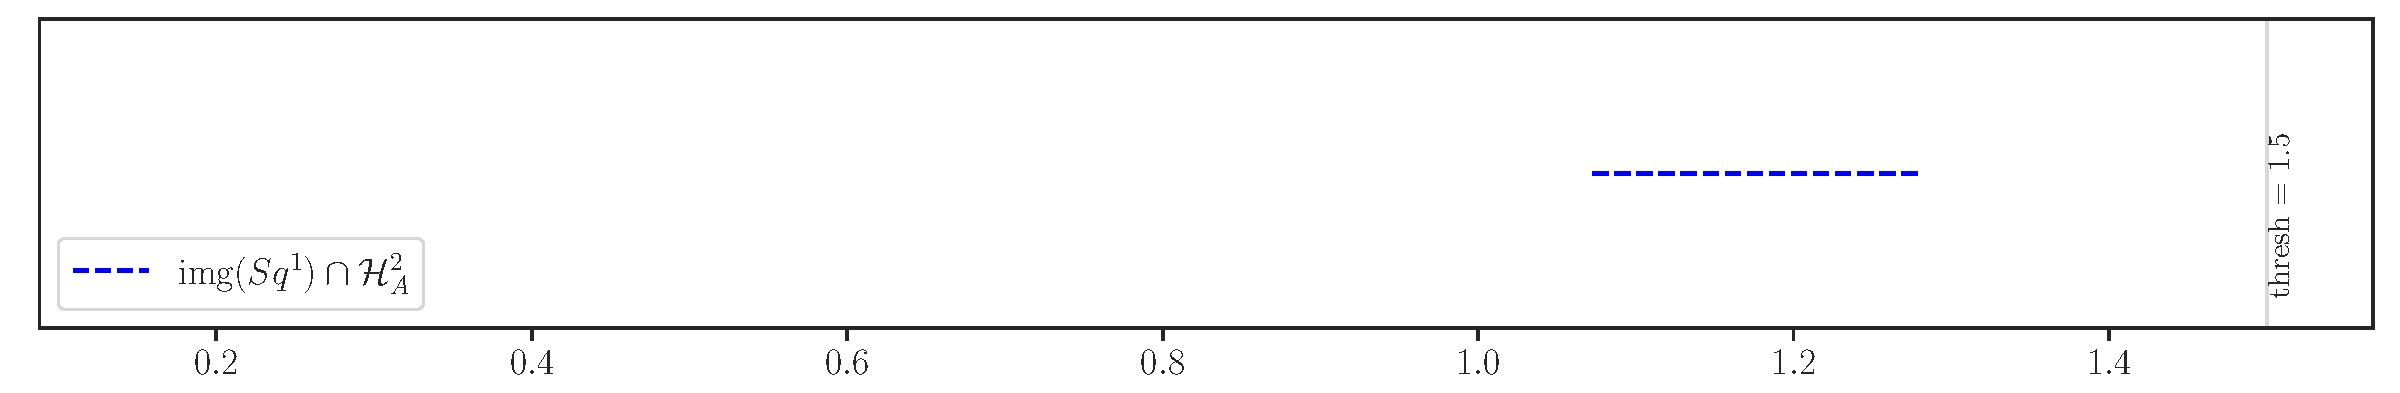
\includegraphics[width=\textwidth]{aux/molecule_bot.pdf}
	Consistent with a \colorit{Klein bottle}.
\end{frame}